\section{Introduction}

This \cgal\ package implements some
of the state-of-the-art surface reconstruction methods. Priority is
given to methods which take as input unorganized point sets and
which compute an implicit function, although we leave the room to
Delaunay-based techniques as all building blocks are available in
\cgal. A common implicit function is an approximate distance function
to the input points or to an estimate tangent plane, or an indicator
function.

The package proposes an interface to the \cgal\ Surface Mesh Generator~\cite{cgal:ry-gsddrm-06,cgal:bo-pgsms-05},
and we leave the room to other surface contouring techniques such
as the Marching Cubes algorithm~\cite{LC87} and its variants (a
user may prefer using his favorite contouring algorithm).

The input is an unorganized point set, possibly with attributes
such as unoriented normals, oriented normals.

Since reconstruction methods often require to preprocess a point set
(e.g. estimate and orient the normals), we provide components devoted
to this task.

The output can be either an implicit function (ready for evaluation
by any contouring algorithm), or a surface mesh, compatible with the
BGL Graph concept and \cgal\ polyhedron when 2-manifold, or represented
as a polygon soup otherwise.

% Insert image introduction.jpg/eps
\begin{center}
    \label{Surface_reconstruction_3-fig-introduction}
    % Image
    \begin{ccTexOnly}
        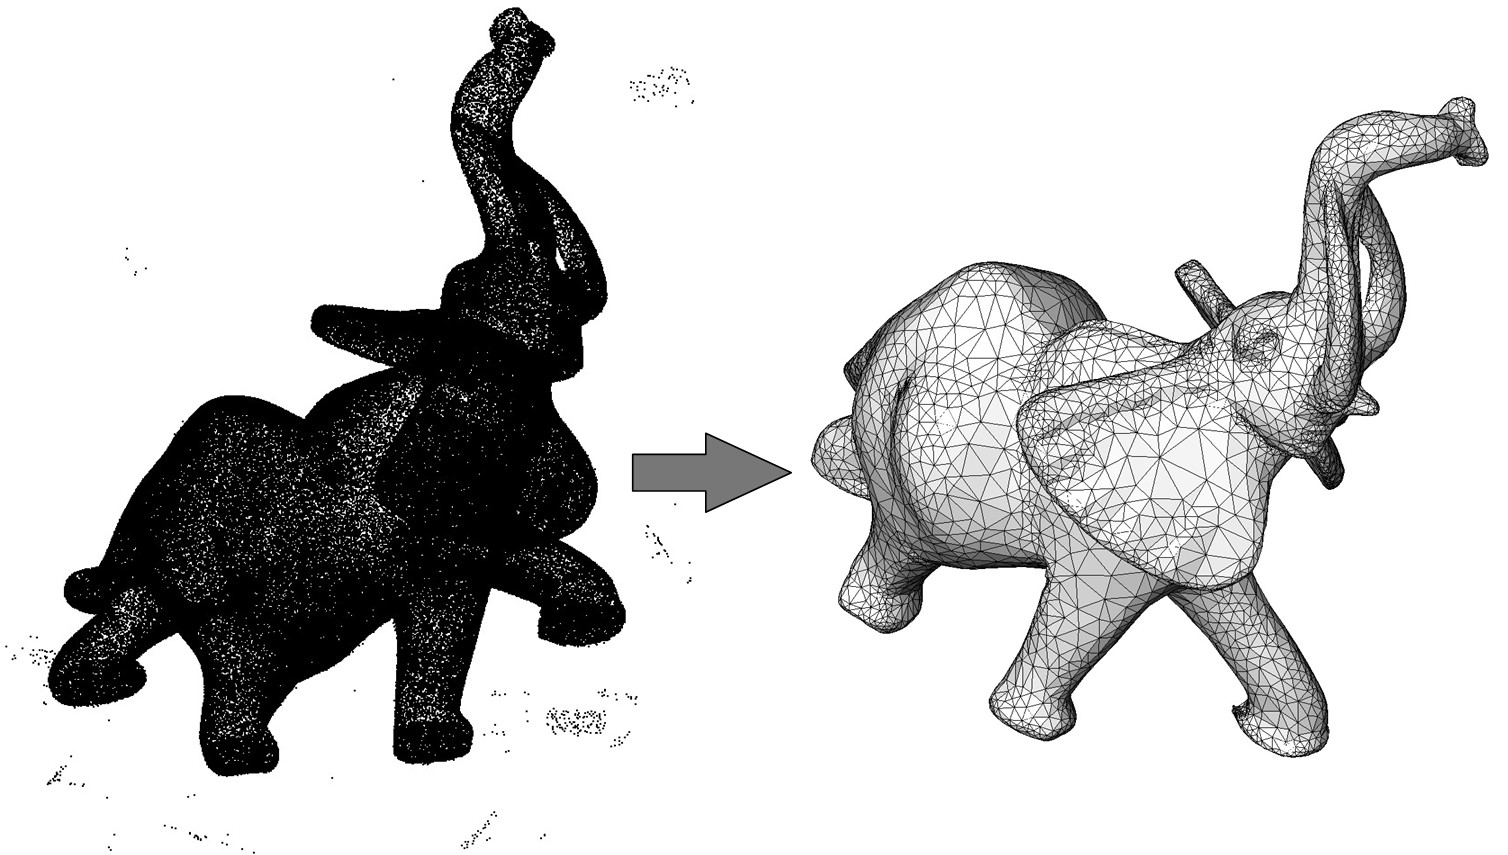
\includegraphics[width=0.9\textwidth]{Surface_reconstruction_3/introduction} % omit .eps suffix
    \end{ccTexOnly}
    \begin{ccHtmlOnly}
        <img width="90%" border=0 src="./introduction.jpg"><P>
    \end{ccHtmlOnly}
    % Title
    \begin{figure}[h]
        \caption{Surface reconstruction from point set}
    \end{figure}
\end{center}


\subsection{Related Work}

\begin{itemize}
\item Taxonomy of reconstruction methods:

\begin{itemize}
\item Based on an implicit function:

\begin{itemize}
\item Signed approximate distance to points \cite{cgal:cl-vmbcm-96}
\item Signed approximate distance to tangent plane estimates \cite{cgal:hddms-srup-92,BC02}
\item RBF \cite{CBC01}
\item Poisson \cite{Kazhdan06}
\item Algebraic Point Set Surfaces \cite{Guennebaud07}
\item ...
\end{itemize}

\item Delaunay-based
\item Deformable models
\item Graph cuts
\end{itemize}

\item Properties of reconstruction methods:

\begin{itemize}
\item Interpolation vs approximation
\item Resilient to noise?
\item Resilient to outliers?
\item Resilient to sparse sampling?
\item Resilient to over-sampling?
\item Resilient to anisotropic sampling?
\item Watertight output?
\item 2-manifold output?
\item Smooth vs piecewise smooth reconstruction?
\item Scalability?
\item Out-of-core/streaming/on-line?
\end{itemize}

\item Taxonomy of normal estimation methods:

\begin{itemize}
\item Point-based Principal Components Analysis over the K nearest neighbors
\item Weighted point-based Principal Components Analysis over the K nearest neighbors
\item Jet fitting
\item Pole-based
\item Voronoi-based Principal Components Analysis
\item ...
\end{itemize}

\item Taxonomy of normal orientation methods:

\begin{itemize}
\item Minimal Spanning Tree \cite{cgal:hddms-srup-92}
\item Pole-based \cite{ABK98,BC02}
\item ...
\end{itemize}

\end{itemize}


\subsection{Overall Package Description}

\subsubsection{Input}

\begin{itemize}
\item 3D points
\item 3D points with unoriented normals
\item 3D points with oriented normals
\end{itemize}


\subsubsection{Analysis}

\begin{itemize}
\item Point set barycenter, bounding box, bounding sphere (provided by \cgal\ Principal Components Analysis package)
\item Average spacing to the K nearest neighbors
\end{itemize}


\subsubsection{Processing}

Outliers removal methods:

\begin{itemize}
\item Outliers removal wrt average squared distance to the K nearest neighbors
\end{itemize}

Point set simplification methods:

\begin{itemize}
\item Point set simplification by clustering
\item Random point set simplification
\end{itemize}

Smoothing methods:

\begin{itemize}
\item Smoothing via Jet fitting over the K nearest neighbors + reprojection
\end{itemize}

Normals estimation methods:

\begin{itemize}
\item Normals estimation by Principal Components Analysis over the K nearest neighbors
\item Normals estimation by Jet fitting over the K nearest neighbors
\end{itemize}

Normals orientation methods:

\begin{itemize}
\item Normals orientation using a Minimal Spanning Tree \cite{cgal:hddms-srup-92}
\end{itemize}


\subsubsection{Surface Reconstruction Methods}

Implicit functions:

\begin{itemize}
\item Delaunay-based Poisson reconstruction \cite{Kazhdan06}
\item Algebraic Point Set Surfaces \cite{Guennebaud07}
\end{itemize}

Implicit function contouring:

\begin{itemize}
\item \cgal\ Surface Mesh Generator~\cite{cgal:ry-gsddrm-06,cgal:bo-pgsms-05}
\end{itemize}


\subsubsection{Output}

\begin{itemize}
\item 2-manifold surfaces vs non-manifold surfaces
\item Watertight models vs models with boundaries
\item The general case is just: a polygon soup
\end{itemize}


